\documentclass[letterpaper,openany,twoside,twocolumn]{book}

\newcommand{\PATH}{../../../}

\usepackage[justified]{\PATH dndtemplate/dnd}

\usepackage{\PATH regions/stylesheets/monster_book_commands}
\usepackage{\PATH regions/stylesheets/regions_stylesheet}
\usepackage{\PATH regions/stylesheets/dungeon_stylesheet}
\usepackage{\PATH regions/stylesheets/monster_stylesheet}
\usepackage{\PATH regions/stylesheets/shadowfy}

\usepackage[english]{babel}
\usepackage[utf8]{inputenc}

\AtBeginDocument{\addtocontents{toc}{\protect\thispagestyle{empty}}}

%\newcommand{\entryfont}{\DndFontStatBlockBody} & uses the default font provided by the LaTeX DnD-Template
\newfontfamily\entryfont{Kalam}[Path=\PATH template/fonts/,Extension=.ttf,UprightFont=Kalam-Regular,BoldFont=Kalam-Bold] % requires XeLaTeX or LuaTeX
\newfontfamily\titlefont{Modesto Bold(2)}[Path=\PATH template/fonts/,Extension=.otf,UprightFont=Modesto Bold(2),BoldFont=Modesto Bold(2)] % requires XeLaTeX or LuaTeX

\begin{document}
	% Titlepage	
	\monstersTitlePage{Fae-Kissed Prairies}{images/titlepage_Fae-Kissed_Prairies.jpg}{0.5cm}{0cm}{height=\paperheight}{https://www.artofmtg.com/art/genesis-ultimatum/}{Genesis Ultimatum MtG Art from Ikoria}{Jason Rainville}{A collection of homebrew monsters found in the Fae-Kissed Prairies}
	
	\tableofcontents
	
	\mainmatter
	
	\graphicspath{{./images},{./monsters/Cobalt_Fox/images}}

\MonsterSheetGeometry

% --------------------------------------------------------------------------------------------------- %
% ################################################################################################### %
% #-#-#-#-#-#-#-#-#-#-#-#-#-#-#-#-# Monster-Sheet  with full Footer #-#-#-#-#-#-#-#-#-#-#-#-#-#-#-#-# %
% ################################################################################################### %
% --------------------------------------------------------------------------------------------------- %

\MonsterFooterGraphic{175pt}{430pt}{Cobalt_Fox.png}{}
\addImageDBEntry{CobaltFox1}{Page \thepage}{Art}{https://www.artofmtg.com/art/flourishing-fox/}{Flourishing Fox MtG Art from Ikoria}{Ilse Gort}%

% Monster stat block
\vspace*{-2.75cm}\begin{DndMonster}[width=0.5\textwidth]{Cobalt Fox}
    \DndMonsterType{Small Fey, chaotic good}

    % If you want to use commas in the key values, enclose the values in braces.
    \DndMonsterBasics[
        armor-class = {12},
        hit-points  = {\DndDice{6d6 + 4}},
        speed       = {40 ft., burrow 10 ft.},
    ]

    \DndMonsterAbilityScores[
        str = 8,
        dex = 18,
        con = 9,
        int = 12,
        wis = 16,
        cha = 14,
    ]

    \DndMonsterDetails[
        saving-throws = {Dex +7, Int +5, Cha +5},
        skills = {Perception +4, Stealth +7},
        %damage-vulnerabilities = {cold},
        %damage-resistances = {bludgeoning, piercing, and slashing from nonmagical attacks},
        %damage-immunities = {cold},
        senses = {darksight 60ft., passive Perception 14},
        %condition-immunities = {frightened, poisoned},
        languages = {Sylvan},
        challenge = 2,
    ]
    
	\DndMonsterAction{Fearsome Agility}
	The Cobalt Fox can take the Dash Action as a Bonus Action. Also, Cobalt Foxes do not trigger opportunity attacks.    
	
	\DndMonsterAction{Keen Hearing and Smell}
	The Cobalt Fox has advantage on Perception checks that rely on hearing or smell.
	
	\DndMonsterAction{Innate Spellcasting}
	The Cobalt Fox can innately cast the following spells, without any components. Its spellcasting ability is Wisdom (spell save DC 14):
	\begin{itemize}
		\item At will: Aid, Cure Wounds
		\item 2/day: Beacon of Hope, Blink
		\item 1/day: Alter Self, Dispel Magic
	\end{itemize}
	
	\DndMonsterAction{Ventriloquism}
	The Cobalt Fox can make its bark (or any sound that it can make) seem to issue from someplace else. With respect to such voices and sounds, anyone who hears the sound can attempt a DC 14 Intelligence (Investigation) check. On success, they recognize it as illusory but still hear it.
    
    \DndMonsterSection{Actions}	
	\DndMonsterAttack[
      name=Bite,
      distance=melee, % valid options are in the set {both,melee,ranged},
      %type=weapon, %valid options are in the set {weapon,spell}
      mod=+2,
      reach=5,
      %range=20/60,
      targets=one target,
      dmg=\DndDice{2d4 + 2},
      dmg-type=piercing,
      %plus-dmg=,
      %plus-dmg-type=,
      %or-dmg=,
      %or-dmg-when=,
      %extra=,
    ]
    
    \DndMonsterAttack[
      name=Gore,
      distance=melee, % valid options are in the set {both,melee,ranged},
      %type=weapon, %valid options are in the set {weapon,spell}
      mod=+4,
      reach=5,
      %range=20/60,
      targets=one target,
      dmg=\DndDice{2d6 + 2},
      dmg-type=piercing,
      %plus-dmg=,
      %plus-dmg-type=,
      %or-dmg=,
      %or-dmg-when=,
      %extra=,
    ]
    
    \DndMonsterAction{Chromatic Burst}
    The fox creates a burst of flickering lights targeting a creature within 30ft. of it. The target must succeed on a DC 13 Wisdom saving throw. On a failed save the target takes \DndDice{2d10 + 4} radiant damage and is blinded until the start of the fox's next turn.
      
\end{DndMonster}

\vfill\eject

\nopagebreakchapter{\hspace*{\columnwidth + 20pt}Cobalt Fox}
\stepcounter{chapter}
\addcontentsline{toc}{chapter}{\protect\numberline{\thechapter}Cobalt Fox}
\vspace*{-6\fontdimen6\font}

\entryfont \noindent \DndDropCapLine{B}looming flower meadows and an abundance of translucent red crystals sprout from the ground. Experienced travellers know they stepped into the territory of Cobalt Foxes. These elusive and magical creatures are distinguished by their dominant gem horn, indistinguishable from the ones spreading throughout their Lair. Although considered a creature of Feywild, they often build their burrows on the Material Plane offering other fey creatures a habitat of their liking.

\DndMonsterAction{Playful but Territorial} The Cobalt Fox itself is appraised as a very intelligent and often supportive fey helping other creatures and humanoids to find there way back to civilization or crucial infrastructure as well as towards feeding and drinking grounds. However, these creature can get highly aggressive and territorial if they sense harm towards their lair and are considered extremely ferocious if their cubs are in danger.\\

\subsection*{Cobalt Fox Lairs}
The presence of this fey fox has an effect on the wilderness around it. The flowers and vegetation is flourishing and seem more vibrant and give off a very strong fragrance. Additionally, small red crystals, so called "fox gems" or "foxes' jewels" are rising up throughout its territory. Not much is known about these crystals, nevertheless a really strong relationship between it and the abilities of Cobalt \linebreak

% --------------------------------------------------------------------------------------------------- %
% ################################################################################################### %
% #-#-#-#-#-#-#-#-#-#-#-#-#-#-# Monster-Sheet with  full Banner-Graphic #-#-#-#-#-#-#-#-#-#-#-#-#-#-# %
% ################################################################################################### %
% --------------------------------------------------------------------------------------------------- %

\MonsterBannerGraphic%
	{}% name of the monster to be displayed as header
	{210pt}% offset for the section header
	{300pt}% max height of the image
	{Cobalt_Fox_Lair.png}% image to be displayed as a banner
	{}% used for keepaspectratio for image ({} or {, keepaspectratio})
	
\addImageDBEntry{CobaltFox2}{Page \thepage}{Background Art}{https://www.artofmtg.com/art/bloodfell-caves-3/}{Bloodfell Caves MtG Art from Ikoria}{Titus Lunter}%
	
Foxes cannot be denied. Studying these crystals turns out to be difficult as they are fiercely defended by the foxes protecting them like their own cub. Therefore, these stones are considered a very coveted magical item.\\
If a pair of Cobalt Foxes build their lair and birth cubs, the territory gets the following Lair Actions.

\subsection*{Lair Actions}
On initiative count 20, any Cobalt Fox considered to be part of the territory takes a lair action to cause one of the following effect. The same effect cannot be used two rounds in a row:
\begin{itemize}
	\item A "fox gem" creates a burst of flickering lights targeting a creature within 10ft. of it. The target must succeed on a DC 12 Wisdom saving throw. On a failed save the target takes \DndDice{1d10} radiant damage and is blinded until the start of the fox's next turn.
	\item A Cobalt Fox within 5ft. of a "fox gem" moves within 5ft. of another "fox gem".
	\item The "fox gem" starts to shimmer. Any creature that isn't a Cobalt Fox has disadvantage on Wisdom and Charisma saving throws until the end of the fox's next turn.
	\item The Zircon Fox can target \DndDice{1d8 + 1} "fox gems" it can see, teleporting to one of them and creating illusions of itself at the others. The illusions have 1 hitpoint and do not make any damage. \textbf{(Only Zircon Fox; 1/Day)}
\end{itemize}

\subsection*{Regional Effects}
The presence of the Cobalt Fox's lair has a slow but steady effect on its surroundings, creating one or more of the following effects:
\begin{itemize}
	\item \textbf{Crystal Profusion.} Natural stone within 500 feet of the lair grows plentiful crystal formations, known as "fox gems".
	\item \textbf{Beautiful Flora.} Flowers and other plants within a 3 miles radius of the lair look especially vibrant and beautiful.
	\item \textbf{Peaceful Atmosphere.} Fey creatures and creatures with fey ancestry within 3 miles of the lair are more at ease and are thus more abundant in the area.
\end{itemize}
If all the Cobalt Foxes die or leave the area, the effects fade over the course of \DndDice{1d10} days.

\vfill\eject

% Monster stat block
\vspace*{-3.1cm}\begin{DndMonster}[width=0.5\textwidth +0.5em]{Zircon Fox}
    \DndMonsterType{Small Fey, chaotic evil}

    % If you want to use commas in the key values, enclose the values in braces.
    \DndMonsterBasics[
        armor-class = {16},
        hit-points  = {\DndDice{14d6 + 10}},
        speed       = {40 ft., burrow 10 ft.},
    ]

    \DndMonsterAbilityScores[
        str = 14,
        dex = 20,
        con = 12,
        int = 14,
        wis = 14,
        cha = 8,
    ]

    \DndMonsterDetails[
        saving-throws = {Dex +9, Int +6},
        skills = {Perception +6, Stealth +9},
        %damage-vulnerabilities = {cold},
        %damage-resistances = {bludgeoning, piercing, and slashing from nonmagical attacks},
        %damage-immunities = {cold},
        senses = {darksight 60ft., passive Perception 14},
        %condition-immunities = {frightened, poisoned},
        languages = {Sylvan},
        challenge = 6,
    ]
    
	\DndMonsterAction{Fearsome Agility}
	The Zircon Fox can take the Dash Action or an Attack Action as a Bonus Action. It does not trigger opportunity attacks.
	
	\DndMonsterAction{Innate Spellcasting}
	The Zircon Fox can innately cast the following spells, without any components. Its spellcasting ability is Wisdom (spell save DC 16):
	\begin{itemize}
		\item At will: Bane, Blur
		\item 3/day: Dispel Magic, Chaos Bolt
		\item 1/day: Antilife Shell, Circle of Death
	\end{itemize}
    
    \DndMonsterSection{Actions}	
	\DndMonsterAttack[
      name=Bite,
      distance=melee, % valid options are in the set {both,melee,ranged},
      %type=weapon, %valid options are in the set {weapon,spell}
      mod=+4,
      reach=5,
      %range=20/60,
      targets=one target,
      dmg=\DndDice{3d8 + 5},
      dmg-type=piercing,
      %plus-dmg=,
      %plus-dmg-type=,
      %or-dmg=,
      %or-dmg-when=,
      %extra=,
    ]
    
    \DndMonsterAttack[
      name=Gore,
      distance=melee, % valid options are in the set {both,melee,ranged},
      %type=weapon, %valid options are in the set {weapon,spell}
      mod=+6,
      reach=5,
      %range=20/60,
      targets=one target,
      dmg=\DndDice{3d10 + 3},
      dmg-type=piercing,
      %plus-dmg=,
      %plus-dmg-type=,
      %or-dmg=,
      %or-dmg-when=,
      extra={. The target must succeed a DC 16 Constitution throw. On a fail the target bleeds.},
    ]
    
    \DndMonsterAction{Achromatic Burst}
    The Zircon Fox creates an aura of darkness targeting a creature within 30ft. of it. The target must succeed on a DC 15 Wisdom saving throw. On a failed saved the target takes \DndDice{4d8 + 8} psychic damage, or half as much on a success, and is frightened by the Zircon Fox until the start of the fox's next turn.
      
\end{DndMonster}

\hspace*{-2.5em}\begin{tabular}{p{0.5\columnwidth}c}
	\MonsterVariantInfoBox{Zircon Fox}{%
		\noindent The Zircon Fox is a much more aggressive and powerful fey creature. It evolves from an orphan cub whose parents were killed. The usual blue fur of a Cobalt Fox becomes red and the most often helpful creature became more treacherous, seeking vengeance on those who mean harm on their kind and territory.
	}
	&
	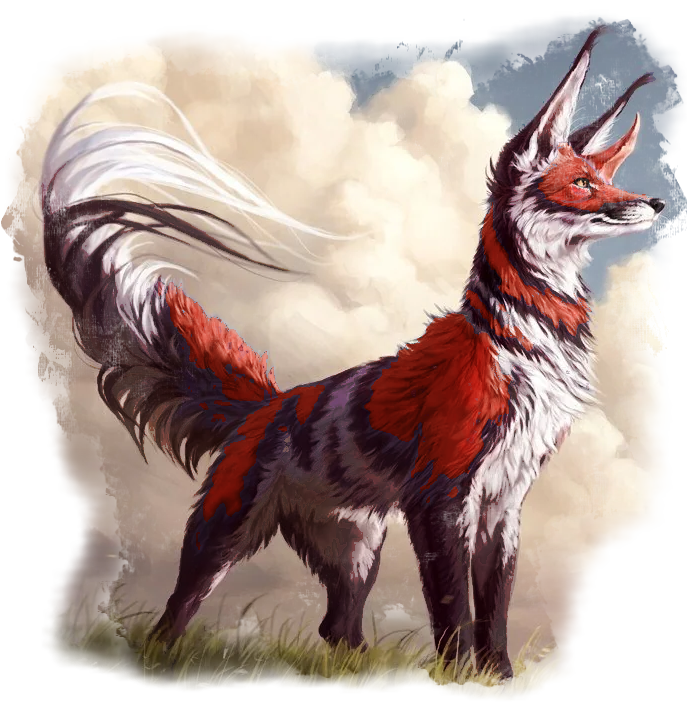
\includegraphics[width=0.65\columnwidth, height=155pt, keepaspectratio]{Zircon_Fox.png}
\end{tabular}
	\graphicspath{{./images},{./monsters/Hypnomoth/images}}

\MonsterSheetGeometry

\newcommand{\artPageCounter}{\thepage}

\chapter*{Hypnomoth}
\stepcounter{chapter}
\addcontentsline{toc}{chapter}{\protect\numberline{\thechapter}Hypnomoth}

\entryfont Within the mystical heart of the Feywild, where reality weaves into enchantment, the Hypnomoth flutters as a living marvel. With wings spanning a meter wide, this wondrous creature dances on the air, its resplendent plumage a dazzling kaleidoscope of colors that defy mortal description. Each wing is a canvas of vibrant hues, intricately adorned with shifting patterns that catch the ambient light and cast shimmering reflections that seem to mirror the very essence of the Feywild itself.

Adorning its head are delicate feelers, like ethereal tendrils of the imagination given form. These adornments quiver and tremble, a sensory extension that captures the enchanting energies of its surroundings. Its six legs end in stingers, a chilling contrast to its bewitching exterior. The stingers gleam like polished daggers, a reminder that beneath the allure lies a creature well-equipped for attack and defense.

The Hypnomoth's flight is a mesmerizing ballet that echoes the harmonious rhythm of the Feywild. It flits through the air with graceful movements, each flutter of its wings a brushstroke upon the canvas of the world. Its presence is a testament to the unbreakable bond between the Feywild's wild magic and the creatures that inhabit it.

\textbf{Colony Gathering} The Hypnomoth makes its home in the heart of the Feywild, where time flows like a river of dreams and the boundaries between reality and imagination blur. It favors the vibrant glades, enchanting meadows, and luminous forests that characterize this realm, where it finds sustenance amidst the Feywild's natural beauty.

While the Hypnomoth is often encountered alone, there are whispered tales of ephemeral gatherings, like moonlit masquerades where these creatures flit and flutter together in dances that are both beguiling and mysterious. These gatherings are rumored to occur during rare celestial events,\linebreak\hspace*{2em}when the boundaries between the Feywild and the\linebreak\hspace*{3.5em}Material Plane are at their thinnest.

\begin{adjustwidth}{0em}{-\linewidth -\columnsep}
\hspace*{5em}\textbf{Charming Presence} Adventurers who cross paths with the\hspace*{22em}\phantom{d}\vspace*{-1.2\fontdimen6\font}\linebreak\hspace*{33.75em}Hypnomoth are simultaneously blessed and\linebreak\hspace*{6.5em}challenged. The creature's enchanting aura is a siren's\hspace*{23em}\phantom{d}\vspace*{-1.2\fontdimen6\font}\linebreak\hspace*{33.4em}call that beckons, tempting those who encounter\linebreak
\end{adjustwidth}


\MonsterGraphicAndShortInfo{shortinfo}% shortinfo or none for no Short-Info Box
{%
	{-1cm}% Shift Horizontal Short Info Box
	{3.9cm}% Shift Vertical Short Info Box
	{-8}% Rotation Angle Short Info Box
	{3.7781cm}% Width of Short-Info Box
	{5}% Number of Lines in Textbox (might be adjusted after 1 compile) 
	{%
		Encountering the Hypnomoth is an experience that weaves the threads of danger and enchantment into a tapestry of wonder.%
	}%
}%
{0.5cm}% Shift Horizontal Monster Grpahic
{0.05cm}% Shift Vertical Monster Grpahic
{, anchor=south west}% Further Picture Placement Options
{(current page.south west)}% Anchor-Point on Page
{height=325pt}% Dimension of Graphic
{Hypnomoth.png}%
\addImageDBEntry{HandleHypnomoth1}{Page \thepage}{Art}{https://www.deviantart.com/davesrightmind/art/Tokyo-SOS-Behemoth-854082946}{Tokyo-SOS-Behemoth}{Davesrightmind}%

\vfill\eject\vspace*{-5.6em}
\begin{DndMonster}[width=0.5\textwidth]{Hypnomoth (Colorful)}
	\DndMonsterType{Large Fey, neutral}
	
	% If you want to use commas in the key values, enclose the values in braces.
	\DndMonsterBasics[
		armor-class = {13 (natural armor)},
		hit-points  = {\DndDice{8d10 + 16}},
		speed       = {20 ft., fly 60 ft.},
	]
	
	\DndMonsterAbilityScores[
		str = 12,
		dex = 16,
		con = 14,
		int = 6,
		wis = 14,
		cha = 10,
	]
	
	\DndMonsterDetails[
		%saving-throws = {Str +0, Dex +0, Con +0, Int +0, Wis +0, Cha +0},
		skills = {Perception +4},
		%damage-vulnerabilities = {cold},
		%damage-resistances = {bludgeoning, piercing, and slashing from nonmagical attacks (not Sandwidow), poison},
		%damage-immunities = {cold},
		senses = {Darkvision 60 ft., passive Perception 14},
		%condition-immunities = {frightened, poisoned, prone},
		languages = {Understands Sylvan but can't speak},
		challenge =5,
	]
	
	\DndMonsterAction{Hypnotic  Aura}
	The Hypnomoth emits an enchanting aura within 30 feet of it. Creatures that start their turn in the aura and can see the Hypnomoth must succeed on a DC 14 Wisdom saving throw or be charmed for 1 minute. A charmed creature is incapacitated and oblivious to danger while charmed. The effect ends if the charmed creature takes damage or if another creature uses an action to shake it out of the trance.
	
	\DndMonsterSection{Actions}
	\DndMonsterAction{Multiattack}
	The Hypnomoth makes three stinger attacks.   
	
	\DndMonsterAttack[
		name=Stinger,
		distance=melee, % valid options are in the set {both,melee,ranged},
		%type=weapon, %valid options are in the set {weapon,spell}
		mod=+5,
		reach=5,
		%range=20/60,
		targets=one target,
		dmg={\DndDice{1d8 + 3}},
		dmg-type=piercing,
		plus-dmg={\DndDice{2d6}},
		plus-dmg-type=poison,
		%or-dmg=,
		%or-dmg-when=,
		%extra=,
	]
	
	\DndMonsterAttack[
		name=Radiant Dart,
		distance=melee, % valid options are in the set {both,melee,ranged},
		%type=weapon, %valid options are in the set {weapon,spell}
		mod=+5,
		reach=120,
		%range=20/60,
		targets=one target,
		dmg={\DndDice{1d12 + 3}},
		dmg-type=radiant,
		%plus-dmg=,
		%plus-dmg-type=,
		%or-dmg=,
		%or-dmg-when=,
		%extra=,
	]
	
	\DndMonsterAction{Color Burst (Recharge 5-6)}
	The Hypnomoth emits an explosion of numerous Radiant Darts, emerging from the Hypnomoth's wings in a 60 foot cone. Each creature in the area of effect must make a DC 14 Dexterity Saving Throw taking \DndDice{5d8} radiant damage on a failed save, or half as much damage on a successful one.  After the Hypnomoth takes this action, it transforms into the Shade version of the Hypnomoth. The hit points and all conditions - except of being poisoned - persist during the form change.
\end{DndMonster}

\vspace*{3\fontdimen6\font}
\noindent \hspace*{4.85em}it to bask in its hypnotic beauty. But this allure\linebreak\hspace*{4.5em}comes with a price, as the moth's powers can\linebreak\hspace*{4.15em}render even the strongest minds vulnerable to its\linebreak\hspace*{3.8em}charms. Those who brave the Hypnomoth's\linebreak\hspace*{3.45em}presence must navigate the boundary between awe\linebreak\hspace*{3em}and peril, for within its mesmerizing display lies the\linebreak\hspace*{2.5em}potential for enchantment and danger alike.

\hspace*{1em}Scholars of the Feywild regard the Hypnomoth as a living\linebreak\hspace*{1.35em}embodiment of the realm's capricious nature. Its vibrant\linebreak\hspace*{0.9em}colors and intoxicating aura serve as a reminder that the\linebreak\hspace*{0.2em}beauty of this plane is often intertwined with hidden threats. Yet, its existence is also a symbol of the Feywild's connection to enchantment and wonder, a living testament to the magic that pulses through every aspect of this realm.

\clearpage

\begin{DndMonster}[width=0.5\textwidth]{Hypnomoth (Shade)}
	\DndMonsterType{Large Fey, neutral}
	
	% If you want to use commas in the key values, enclose the values in braces.
	\DndMonsterBasics[
		armor-class = {16 (natural armor)},
		hit-points  = {\DndDice{8d10 + 16}},
		speed       = {20 ft., fly 60 ft.},
	]
	
	\DndMonsterAbilityScores[
		str = 14,
		dex = 14,
		con = 14,
		int = 6,
		wis = 16,
		cha = 8,
	]
	
	\DndMonsterDetails[
		%saving-throws = {Str +0, Dex +0, Con +0, Int +0, Wis +0, Cha +0},
		skills = {Perception +5},
		%damage-vulnerabilities = {cold},
		%damage-resistances = {bludgeoning, piercing, and slashing from nonmagical attacks (not Sandwidow), poison},
		%damage-immunities = {cold},
		senses = {Darkvision 60 ft., passive Perception 15},
		condition-immunities = {Poisoned},
		languages = {Understands Sylvan but can't speak},
		challenge =5,
	]
	
	\DndMonsterAction{Ethereal Siphon}
	The Hypnomoth gains a Color counter each time it successfully uses its Chromavore ability. When its Color counter reaches a number equal to its Challenge Rating, it transforms back into the Colorful version of the Hypnomoth.
	
	\DndMonsterAction{Chromavore}
	Whenever the Chromatic Tail Stinger attack hits, the target must make a DC 12 Constitution saving throw. On a failed save, the target's body is drained of color, leaving it visually muted and monochromatic. The target becomes affected by Monochromatism and takes \DndDice{1d8} necrotic damage. The Hypnomoth gains one Color counter.
	
	\DndMonsterAction{Ethereal Cloak}
	The Hypnomoth gains partial incorporeality, allowing it to move through objects and avoid physical harm. Attacks against it that rely on non-magical weapons have disadvantage. 
	
	\DndMonsterSection{Actions}
	
	\DndMonsterAttack[
		name=Bloodsucking Beak,
		distance=melee, % valid options are in the set {both,melee,ranged},
		%type=weapon, %valid options are in the set {weapon,spell}
		mod=+4,
		reach=5,
		%range=20/60,
		targets=one target,
		dmg={\DndDice{2d10 + 2}},
		dmg-type=piercing,
		%plus-dmg=,
		%plus-dmg-type=,
		%or-dmg=,
		%or-dmg-when=,
		extra={, and the Hypnomoth regains hit points equal to half the damage dealt.},
	]
	
	\DndMonsterAttack[
		name=Stinger Strike,
		distance=melee, % valid options are in the set {both,melee,ranged},
		%type=weapon, %valid options are in the set {weapon,spell}
		mod=+4,
		reach=5,
		%range=20/60,
		targets=one target,
		dmg={\DndDice{1d4 + 2}},
		dmg-type=radiant,
		plus-dmg=\DndDice{2d6},
		plus-dmg-type=poison,
		%or-dmg=,
		%or-dmg-when=,
		extra={. The target must succeed on a DC 14 Constitution saving throw or be poisoned for 1 minute. The creature can repeat the saving throw at the end of each of its turns, ending the effect on a success.},
	]
	
	\DndMonsterAttack[
		name=Chromatic Tail Stinger,
		distance=melee, % valid options are in the set {both,melee,ranged},
		%type=weapon, %valid options are in the set {weapon,spell}
		mod=+3,
		reach=5,
		%range=20/60,
		targets=one target,
		dmg={\DndDice{1d4 + 3}},
		dmg-type=piercing,
		%plus-dmg=,
		%plus-dmg-type=,
		%or-dmg=,
		%or-dmg-when=,
		%extra={},
	]
	
	\DndMonsterSection{Reactions}
	\DndMonsterAction{Lightning Tail Whip}
	Whenever the Hypnomoth's (Shade) hits a target with a melee attack or is attacked by a melee attack it can use its Reaction to make a Chromatic Tail Stinger Attack on the other creature.
\end{DndMonster}

\MonsterGraphicAndShortInfo{}% shortinfo or none for no Short-Info Box
{}%
{0.25cm}% Shift Horizontal Monster Grpahic
{0.05cm}% Shift Vertical Monster Grpahic
{, anchor=north east}% Further Picture Placement Options
{(current page.north east)}% Anchor-Point on Page
{height=360pt}% Dimension of Graphic
{Hypnomoth_Shade.png}%
\addImageDBEntry{HandleHypnomoth2}{Page \thepage}{Art}{https://www.deviantart.com/davesrightmind/art/Adult-Spear-Fly-879317343}{Adult Spear Fly}{Davesrightmind}%
\vspace*{-1.2\fontdimen6\font}
\section*{The Shade's Unveiling}
\addcontentsline{toc}{section}{The Shade's Unveiling}
As the radiant burst reaches its zenith and the darts disperse into the air, a subtle yet profound shift begins to weave its magic. The once-vibrant colors that adorned the Hypnomoth's wings, each a brushstroke of the Feywild's enigmatic palette, start to ebb away. In their wake emerges a spectral pallor, a gossamer cloak of hues that shimmers with a delicate translucence. Each hue fades like the receding echoes of an ancient melody, leaving behind a canvas of twilight beauty.
\vfill\eject
\noindent From within the radiant aftermath\\of the burst and amidst the spectral\\luminescence, the Hypnomoth's\\metamorphosis concludes.\\Emerging from the depths\\of shimmering radiance,\\the creature reveals its\\new incarnation - the\\Shade version of the\\Hypnomoth. The vibrant\\colors that once danced\\upon its wings now yield\\to a pale, ghostly trans-\\lucence, akin to the delicate\\wings of a moth caught\\between moonbeams. Its\\form resonates with an\\enigmatic allure that hints\\at the very essence of the\\Feywild's mysteries.
\\\\
\paragraph*{Behavior and Impact}\hfill\\
The Shade Hypnomoth's\\behavior takes on an otherworldly demeanor.\\It moves with a quiet grace, its wingbeats barely\\audible as it drifts through the air like a specter. Rather than drawing attention with vibrant displays, it maintains a somber elegance, as if acknowledging its altered presence within the realm.

The creature's Chromavore ability reveals its inscrutable nature. Engaging in its unique form of feeding, it drains the color from its foes, leaving them muted and devoid of life's vibrancy. As it gathers these chromatic essences, its own spectral form seems to intensify, as if empowered by the very shades it consumes.

The impact on its environment is both subtle and profound. Creatures within its vicinity often display signs of unease, as if the natural hues around them have dimmed in the Hypnomoth's presence. Vegetation loses a fraction of its lushness, and the world seems to momentarily hold its breath in acknowledgment of the creature's ethereal essence.
\\
\subsubsection*{Effect of Monochromatism}
The absence of vibrant colors and the muted palette detract from a creature's ability to express emotions and intentions through visual cues. This leads to a disadvantage on Charisma-based ability checks, as their communication becomes less engaging and relatable.

Restoring a creature's lost color is no simple feat, as the Chromavore's effects run deeper than mere physical appearance. It requires the performance of the Chromatic Restoration Ritual which utilizes the delicate wings of the Hypnomoth as a key ingredient which must be bathed in moonlight thus restoring the color of the affected partaking in the ritual.
	
	% Final Page
	\monstersLastPage{images/backcover_Fae-Kissed_Prairies.jpg}{0cm}{3cm}{height=\paperheight}{https://www.worldanvil.com/media/cache/cover/uploads/images/d778432f3604f389555b172d4adb69da.jpg}{The Feywild}{Worldanvil}{}
\end{document}